\documentclass[10pt, a4paper]{article}
\usepackage[a4paper,outer=1.5cm,inner=1.5cm,top=1.75cm,bottom=1.5cm]{geometry}

\twocolumn
\usepackage{graphicx}

\usepackage{hyperref}
\usepackage[utf8]{inputenc}
\usepackage{amsmath}
\usepackage{physics}
\usepackage{amssymb}
\begin{document}
\title{Properties of Collinear (Assignment-3)}
\date{}
\maketitle

\begin{center}
\title{\textbf{}}
\date{\vspace{-5ex}} %Not to print date automatically
\maketitle
\end{center}

\setcounter{page}{1}

\section{10$^{th}$ Maths - Chapter 7}

This is Problem-2 from Exercise 7.3.2

\section{Problem } 
In Each of the following find the value of k, for which the point of collinear (1)( (7, -2),(5, 1),(3, k) (2)(8,1),(k,-4),(2,-5).\\
\section{Solution for problem 1}
\begin{center}
The input given 
\boldmath
\begin{equation} \label{eq:}
A=\begin{pmatrix} 7\\ -2\ \end{pmatrix} 
\end{equation}
\begin{equation}\label{eq:}
B=\begin{pmatrix} 5\\ 1\ \end{pmatrix}
\end{equation}
\begin{equation}\label{eq:}
C=\begin{pmatrix} 3\\ 4\ \end{pmatrix}
\end{equation}
\unboldmath
\end{center}
\begin{equation}\label{eq:}
\textbf{D=A-B}\\
=\begin{pmatrix} 7\\ -2\ \end{pmatrix}- \begin{pmatrix} 5\\ 1\ \end{pmatrix}
\end{equation}
\begin{equation}\label{eq:}
=\begin{pmatrix} 2\\ -3\ \end{pmatrix}\\
\end{equation}
\begin{equation}\label{eq:}
\textbf{E=A-C}\\
=\begin{pmatrix} 7\\ -2\ \end{pmatrix}- \begin{pmatrix} 3\\ k\ \end{pmatrix}
\end{equation}
\begin{equation}\label{eq:}
=\begin{pmatrix} 4\\ -2-k\ \end{pmatrix}\\
\end{equation}
\boldmath
Now the matrix is\\
\begin{equation}\label{eq:}
\textbf{F=$\begin{pmatrix} D\\ E\ \end{pmatrix}$}
\end{equation}
\unboldmath
\begin{equation} \label{eq:}
=\begin{pmatrix} 2 & -3\\ 4 & -2-k \ \end{pmatrix} 
\end{equation}
If  points on a line  are  collinear, rank of matrix is " 1 "then the vectors are in linearlydependent.
For 2 × 2 matrix Rank =1 means Determinant is 0.

Through pivoting,we obtain\\
\begin{equation}\label{eq:}
=\begin{pmatrix} 2 & -3\\ 4 & -2-k \ \end{pmatrix} \\ 
\end{equation}
\begin{equation}\label{eq:}
=\begin{pmatrix}
2 &-3 \\ 
 4& -2-k
\end{pmatrix}\overset{R2=R2-R1}{\rightarrow}
=\begin{pmatrix}
-2-k &-4 \\ 
 4& -2-k
\end{pmatrix}
\end{equation} 
if the rank of the matrix is 1 means any one of the row must be zero.So, making the first element in the matrix to 0.
\begin{equation}\label{eq:}
-2-k-2(-3)=0
\end{equation} 
\begin{equation}\label{eq:}
-2-k-6=0\\
\end{equation} 
\begin{equation}\label{eq:}
k=4 \\
\end{equation} 
Hence proved.

 \begin{figure}[h!]
	  \centering 
	  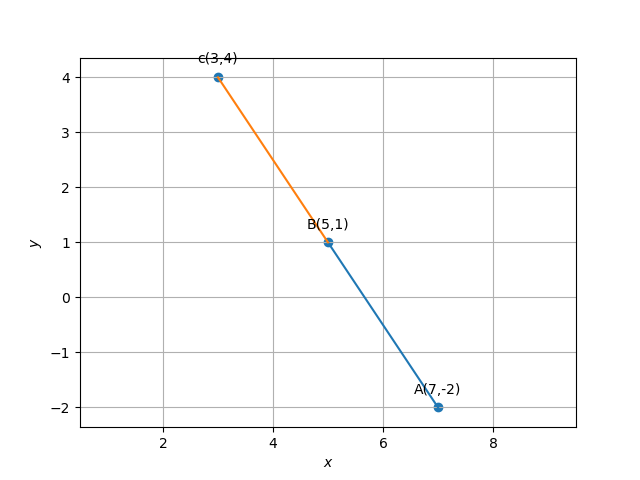
\includegraphics[width=\columnwidth]{line1.png}
	  \caption{}
	  \label{fig:line.png}
\end{figure}
\section{Solution for problem 2}
\begin{center}
The input given 
\boldmath
\begin{equation} \label{eq:}
A=\begin{pmatrix} 8\\ 1\ \end{pmatrix} 
\end{equation}
\begin{equation}\label{eq:}
B=\begin{pmatrix} k\\ -4\ \end{pmatrix}
\end{equation}
\begin{equation}\label{eq:}
C=\begin{pmatrix} 2\\ -5\ \end{pmatrix}
\end{equation}
\unboldmath
\end{center}
\begin{equation}\label{eq:}
\textbf{D=A-B}\\
=\begin{pmatrix} 8\\ 1\ \end{pmatrix}- \begin{pmatrix} k\\ -4\ \end{pmatrix}
\end{equation}
\begin{equation}\label{eq:}
=\begin{pmatrix} 8-k\\ 5\ \end{pmatrix}\\
\end{equation}
\begin{equation}\label{eq:}
\textbf{E=A-C}\\
=\begin{pmatrix} 8\\ 1\ \end{pmatrix}- \begin{pmatrix} 2\\ -5\ \end{pmatrix}
\end{equation}
\begin{equation}\label{eq:}
=\begin{pmatrix} 6\\ 6\ \end{pmatrix}\\
\end{equation}
\boldmath
Now the matrix is\\
\begin{equation}\label{eq:}
\textbf{F=$\begin{pmatrix} D\\ E\ \end{pmatrix}$}
\end{equation}
\unboldmath
\begin{equation} \label{eq:}
=\begin{pmatrix} 8-k & 5\\ 6 & 6 \ \end{pmatrix} 
\end{equation}
If  points on a line  are  collinear, rank of matrix is " 1 "then the vectors are in linearlydependent.
For 2 × 2 matrix Rank =1 means Determinant is 0.
hrough pivoting,we obtain
\begin{equation}\label{eq:}
=\begin{pmatrix} 8-k & 5\\ 6 & 6 \ \end{pmatrix} \\ 
\end{equation}
\begin{equation}\label{eq:}
=\begin{pmatrix}
8-k & 5 \\ 
 6& 6
\end{pmatrix}\overset{R1=3R1-3R2}{\rightarrow}
=\begin{pmatrix}
24-3k &15 \\ 
 6& 6
\end{pmatrix}
\end{equation}

if the rank of the matrix is 1 means any one of the row must be zero.So, making the first element in the matrix to 0.
\begin{equation}\label{eq:}
3(8-k)-3(5)=0
\end{equation} 
\begin{equation}\label{eq:}
24-3k-15=0\\
\end{equation} 
\begin{equation}\label{eq:}
k=3 \\
\end{equation} 
Hence proved.
\begin{figure}[h!]
	  \centering 
	  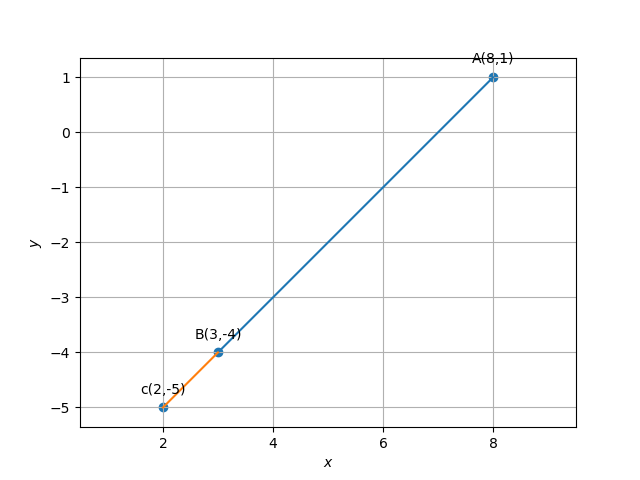
\includegraphics[width=\columnwidth]{line2.png}
	  \caption{}
	  \label{fig:line2.png}
	  \end{figure}

\end{document}
